\documentclass{article}
\usepackage{graphicx}
\usepackage{amsmath}
\usepackage{hyperref}
\usepackage{physics}
\usepackage{cleveref}
\usepackage{titling}
\usepackage[a4paper, margin=3.5cm]{geometry}
\usepackage{fontspec}
\usepackage{indentfirst}
\usepackage{float}


\setmainfont{Times New Roman}
\bibliographystyle{unsrt}
\title{\textbf{Report on the hierarchical Ising opinion model}}
\setlength{\droptitle}{-3cm} 
\date{}


\begin{document}
\maketitle

\section{Introduction}
Polarization is becoming a common social phenomenon in recent years\cite{abramowitz2008polarization}. After a series of interactions, 
including exposure under contrary opinions\cite{bail2018exposure} and discussions within group with similar opinions\cite{smith2024polarization},
their opinions toward an attitude object tend to polarize further. Such phenomena increase opposition and prevent reaching a cooperation, which is impactful
in social issues. Hence, studying the formation of polarization is a crucial topic in sociology.\\

The journal article "\textit{The polarization within and across individuals: the hierarchical Ising opinion model}"\cite{van2020polarization} proposed a 
HIOM (hierarchical Ising opinion model) to simulate the evolution of polarization in a group of people. The model successfully predicts the polarization effects
and gives an explanation base on the cusp catastrophe due to Ising model. The article not only reproduces an empirical case of polarization, but also provides a method to 
reduce the degree of polarization on an attitude object, which is potentially useful in understanding the polarization phenomenon.\\

The report aims to look further into the HIOM and its simulation results in order to have a deeper understanding in the implication and mechanism of the model
parameters. Several insights were raised and aim to complement the original study, and were inspiring enough to develop new method to reduce polarization by making use of 
the mechanisms. In addition, the effect of diffusion of opinion by activists is explored.\\

The report is organized as follows. The HIOM is first explained in detail, then the results produced by the article will be explained and as supplement to
the article's findings. At last, the effect of opinion diffusion will be shown and discussed.

\section{Methods}
The HIOM consists of two levels, the individual level and the interpersonal level. The individual one incorporates some features of the classical Ising model,
which is originally about the collective ferromagnetic behavior of a material arising from spin of particles in a lattice\cite{budrikis2024100}, 
to describe the opinion evolution in an agent. While the interpersonal one focuses on the interaction between agents.

\subsection{Individual level of HIOM}
The individual level of HIOM, referred to as the Ising attitude model in the article, is a network constituted by many interacting attitude element nodes. These 
nodes could be about feelings, behaviors and beliefs. When an attitude object is raised, a certain combination of nodes that are related to the attitude object
will be activated, and the collective behavior of these nodes determines the opinion of an agent.

\subsubsection{Glauber dynamics}
Glauber dynamics is a kind of Monte Carlo method (simulating complex system by random numbers), which is used to simulate the classical Ising model on a computer. In Glauber dynamics, the energy
of Ising model system is given by the Hamiltonian\cite{cipra1987introduction,brush1967history}:

\begin{equation}
    H(x) = -\sum_i \tau_i x_i -\sum_{\langle i,j \rangle} \omega_{ij}x_ix_j
\end{equation}

Where $x_i$ is the spin of a particle on the lattice network, $\tau_i$ is the external field strength and $\omega_{ij}$ is the interacting parameter. In some simplification, the
interacting parameter and external field strength is often a constant. For Glauber dynamics, the algorithm
goes as following\cite{walter2015introduction}:
\begin{enumerate}
    \item Select a particle randomly.
    \item Calculate energy difference $\Delta H = H_{new} - H_{old}$ of the system if the spin of that particle is flipping.
    \item Flip the spin according to the probability $P_{flip} = \frac{1}{1+e^{\frac{\Delta H}{kT}}}$, where $T$ is temperature and $k$ is Boltzmann constant.
    \item Repeat from step 1.
\end{enumerate}
The Ising attitude model follows Glauber dynamics, and connect it with human psychological activity though four assumptions. Which means the meaning of parameters
such as $x_i, \omega_{ij}, \tau_i, \frac{1}{kT}$ have to be explained.

\subsubsection{Assumptions}
The first assumption is that the nodes can be described by a binary variable, which can be denoted as $x_i \in \{-1,+1\}$ ($i\;in\;1...n$), representing a pair of opposite states. The states are related
to stances toward an attitude object, for example, in a topic like vegetarian or meat-eater, +1 in a node about feeling (taste of meat) could means tasty, while
-1 means the opposite. The sum of $x_i$ defines the opinion of an agent. Hence we have opinion $O = \sum_i^nx_i$, and we interpret positive and negative values as two 
contrary stance, while the magnitude represent the degree.\\

The second assumption is that the connections between nodes are symmetric, which means the connection weights $\omega_{ij}$ are always the same between a pair 
of particular nodes no matter the direction. The attitude element nodes can affect each other just like feeling (animals are cute) can affect behavior (eat meat),
and two connected nodes always influence each other equally.\\

The third assumption is that the nodes possess inherent disposition $\tau_i$, which associate with the probability of the node adopting +1 or -1 state without
any influence from other nodes. $\tau_i \in (-\infty,+\infty)$ can be projected to a value of probability in $[0,1]$ by a function in the form $f(\tau_i) = \frac{1}{1+a^{-b\tau_i}}$, where $a$ 
and $b$ are just some parameters to control the steepness of the function. The reason of choosing whole real range for $\tau_i$ is to provide a larger flexibility for HIOM. Dispositions here to Ising attitude model is just what external field strength to classical Ising model\cite{cipra1987introduction},
which could represent including the social influence (values, ethics) and inborn nature, in situation like a society. To summarize the mean effect of disposition,
we have $I = \bar{\tau}$, which is the mean value of $\tau$.\\

In the fourth assumption, attention $A$ (usually $A>0$), which is a parameter, was introduced to replace inverse of temperature and Boltzmann constant, $A = \frac{1}{kT}$. Attention tells how sensitive a node will be influenced by other nodes. If attention is
high, a node tends to be affected by the network environment easily and show consistency with other nodes. An attention of 0 means completely random behavior of a node, which has no relevance with the network.
The attention assumption likely emerged to align with the algorithm of Glauber dynamics, so that the attention is analogous to the 
inverse of temperature and Boltzmann constant in the spin flip probability of Glauber dynamics. Apart from that, interpreting it as how agents think about an attitude object
is also intuitive. If one thinks more on a topic (high $A$), his nodes flip purposefully and will probably develop a certain stance, if one does not think about a topic (low $A$ or $A=0$),
his nodes flip randomly that he is not likely to have a clear stance.

\begin{figure}[htbp]
    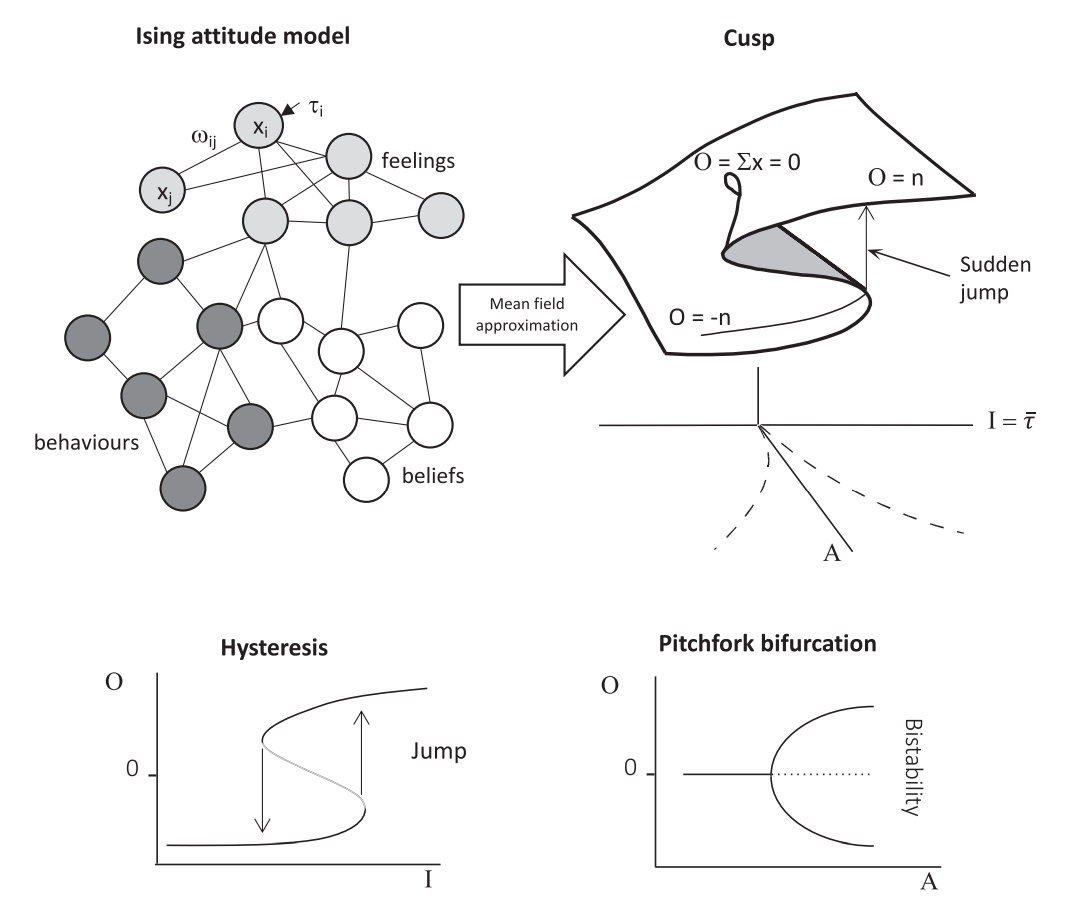
\includegraphics[width = 0.7\textwidth]{misc figure/isingattitudemodel.png}
    \centering
    \caption{Figure from\cite{van2020polarization}. The upper part shows after mean field approximation of Ising model, the cusp catastrophe graph can be constructed, the surface is just the equilibrium state of the system. The lower left figure shows hysteresis at a fixed $A$, while right figure show bifurcation of equilibrium position along fixed $I$.}
    \label{fig1}
\end{figure}
\subsubsection{Cusp catastrophe}
It is easy to understand that the Ising attitude model is simply a psychological reinterpretation of the traditional Ising model by stating some assumptions. Apparently,
the Ising attitude model shows similar properties to the classical Ising model. The critical one here is the cusp catastrophe. By mean field approximation, the equilibrium
state of Ising attitude model can be described by an equation\cite{friedli2018statistical,van2020polarization}:
\begin{equation}\label{eq1}
    O^3-AO-I=0
\end{equation}
which is a surface in 3D space with $O,I,A$ as parameter (see \autoref{fig1}). In fact,\autoref{eq1} is a result telling the stationary point of a potential energy function $V(O) = \frac{1}{4}O^4 - \frac{A}{2}O^2 - IO$ in dynamic system.
To find the stationary point, we let $\frac{dV}{dO} = 0$ to obtain \autoref{eq1}. To find the rate of change of O, we can consider that the system tends to minimize its potential energy by changing O,
the moving direction of $O$ should always point to a local minimum of $V(O)$, so we can have a gradient descent relationship $\frac{dO}{dt} = -\frac{dV}{dO}$ (see \autoref{fig3}).
\begin{figure}[H]
    \centering
    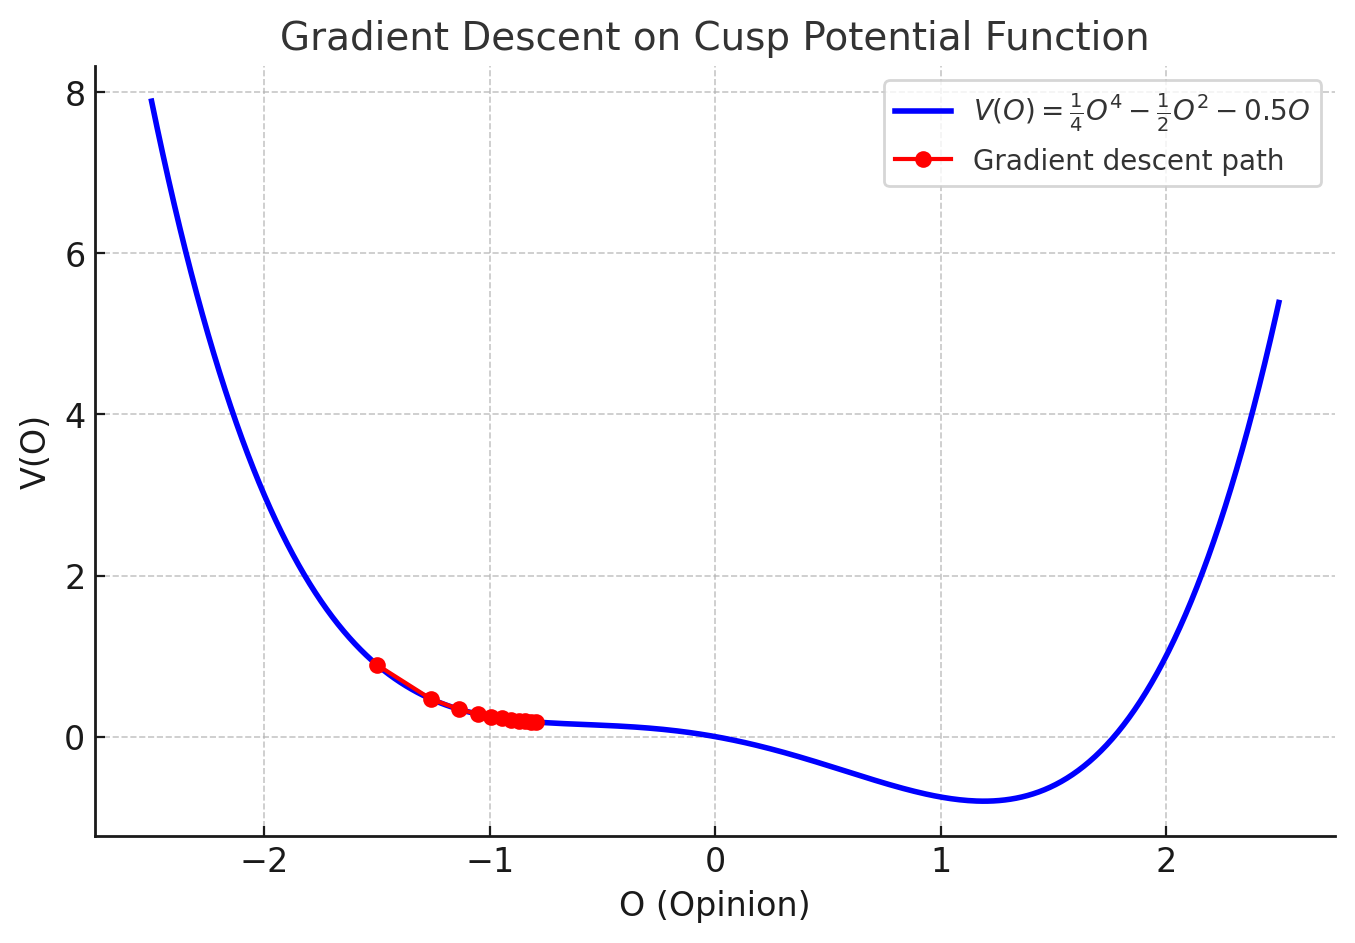
\includegraphics[width=0.5\textwidth]{misc figure/gradientdescent.png}
    \caption{The red dot moving to local minimum at a rate according to slope of $V(O)$ at that point.}
    \label{fig3}
\end{figure}

So we obtain a differential equation $dO = -(O^3-AO-I)dt$ describing rate of change of $O$. For agents at any point in the $O,I,A$ space, they tend to move to the stable equilibrium surface. Note that for area with three stationary position,
the middle one is always an unstable stationary position. The movement of agents in the cusp catastrophe is described in \autoref{fig2}. We can observe that agents are likely to stick 
to the equilibrium surface while changing $I$ and $A$, hence hysteresis and bifurcation of equilibrium appear naturally.\\

\begin{figure}[htbp]
    \centering
    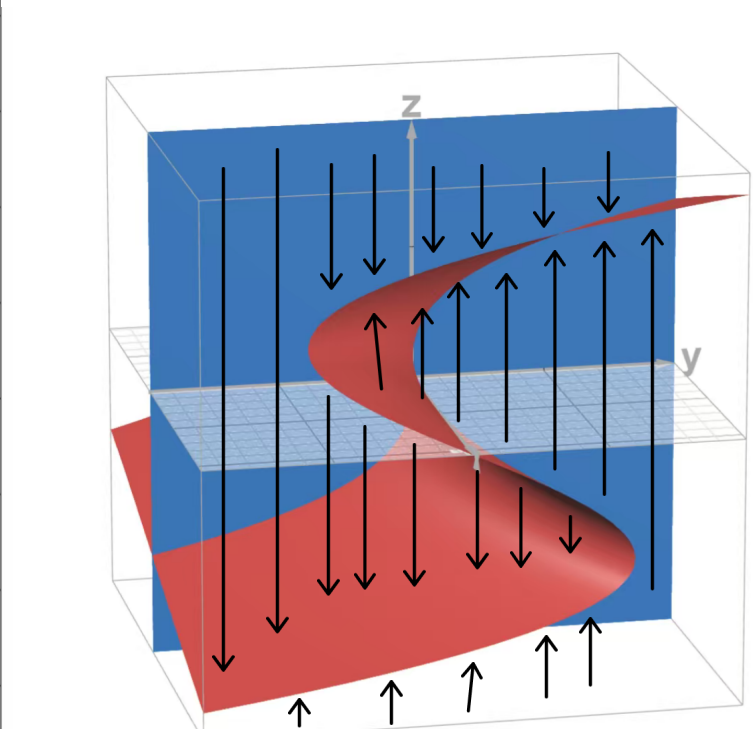
\includegraphics[width=0.4\textwidth]{misc figure/cuspflow.png}
    \caption{Moving direction of agents in the space.}
    \label{fig2}
\end{figure}


\subsection{The HIOM}
The individual level of HIOM concludes the dynamic rules of $O$, while the interperson level of HIOM gives the update mechanism of $I,A$. Together with interaction
between agents, the HIOM is then complete. In HIOM, agents form a network that can interact with each other, leads to update of their own $I$ and $A$, which then
update their $O$.\\

In actual simulation, rate of change of $O$ in each agent ($i...n$) is modified to have better performance, which is:
\begin{equation}\label{eq2}
    dO_i = -(O_i^3 - (A_i+A_{min})O_i - I_i)dt + n_o
\end{equation}
Where $A_{min}$ is a negative number (usually -0.5) introduced to provide linear behavior of $O$ when $A$ is low, and $n_o$ is random noise, equal to the standard deviation of randomly selected numbers in a normal distribution with mean $=0$.\\

The HIOM assumes that the probability of an agent begin an interaction depends on his attention, which means agents with high attention are more likely to start
an interaction. The probability of choosing an agent $i$ to start an interaction is:
\begin{equation}\label{eq3}
    P_i = \frac{A_i}{\sum_iA_i}
\end{equation}

HIOM also assumes that the attention of an agent increase upon successful interaction, and decrease spontaneously with time. The rate of change of attention is:
\begin{equation}\label{eq4}
    dA_i = -\frac{2d_A}{N}A_i + d_A(2A^*-A_i)\delta
\end{equation}
Where $d_A$ controls rate of change of A, $N$ is the number of agents in the network, $A^*$ is the equilibrium position of attention of whole network. If the sample size is large, each agent would have lower chance to be selected and increase their attention, hence $N$ is appeared as the denominator in the decay term
to make sure the overall attention decay is not too violent in any sample size. In every iteration, if the agent interact successfully, then $\delta =1$, otherwise, $\delta = 0$.\\

In each iteration, information $I$ will be updated among agents who involved in an interaction according to:
\begin{equation}\label{eq5}
    I_{i+1} = rI_i + (1 - r)I_j + n_s,\;where\;r = r_{min} +\frac{1-r_{min}}{1+e^{-p(A_i-A_j)}}
\end{equation}
$n_s$ is the noise, which equal to the standard deviation of randomly selected numbers in a normal distribution with mean $=0$ in each update, and $p$ is a parameter reflecting the persuasive strength during interactions of all agents. $r_{min} \in [0,1]$ is a parameter imply the inherent resistance to persuasion of all agents. When both agents have the same attention and $r_{min}=0$,
their updated information will be the mean of their previous information, thus we can infer that agents with higher attention tend to drag the information of their
opponents towards themselves more.\\

The individual level and interpersonal level of HIOM can be conclude easily. The former determines update of opinion while the latter determines update of information and attention.
Combination of them forms a complete dynamic system that we can observe how agents move in the $O,I,A$ space under different circumstances.

\subsection{Measures}
Some quantification methods are employed to evaluate the result. The proportion of positive opinion $p(O>0)$ indicate the distribution of opinions, and the Hartigan D value shows the polarization. Hartigan Dip statistic is used to measure the degree a distribution deflection from a unimodal distribution.
To calculate the Hartigan Dip statistic of a distribution, we convert the distribution into empirical distribution function, and compare its largest vertical difference with each possible unimodal cumulative distribution. Then,
we choose the minimum largest vertical difference among all unimodal cumulative distribution to be the Hartigan Dip statistic value\cite{hartigan1985dip}. So a smaller Hartigan D value means the distribution is more likely to be unimodal.

\subsection{simulation}
The HIOM algorithm in R code is as follow.
\begin{enumerate}
    \item Choose a network topology.
    \item Initialize parameters $N,A_{min},A^*, n_o, n_s, d_A, p, r_{min}, t_o, dt,O,I,A$. Commonly, $dt=0.01,A_{min}=-0.5$, and $t_o$ is bounded confidence.
    \item Begin iteration.
    \begin{enumerate}
        \item Choose an agent according to \autoref{eq3}.
        \item Randomly choose a neighbour as partner for interaction.
        \item If opinion difference is less than $t_o$:
        \begin{enumerate}
            \item Add attention to both agents ($+d_A(2A^*-A_i)\delta$).
            \item Update information by \autoref{eq5}.
        \end{enumerate}
        \item Implement attention decay to all agents ($-\frac{2d_A}{N}A_i$).
        \item Update opinion on all agents by \autoref{eq2}
    \end{enumerate}
\end{enumerate}
    
The code for simulation is available here \url{https://github.com/ASTRAEL-BAI/HIOM-test}.

\section{Extended analysis}\label{Ext}
There are some interesting observations of the HIOM that give us clues in understanding the model, these include noise, the information parameter and the attention parameter.\\

\begin{figure}[H]
    \centering
    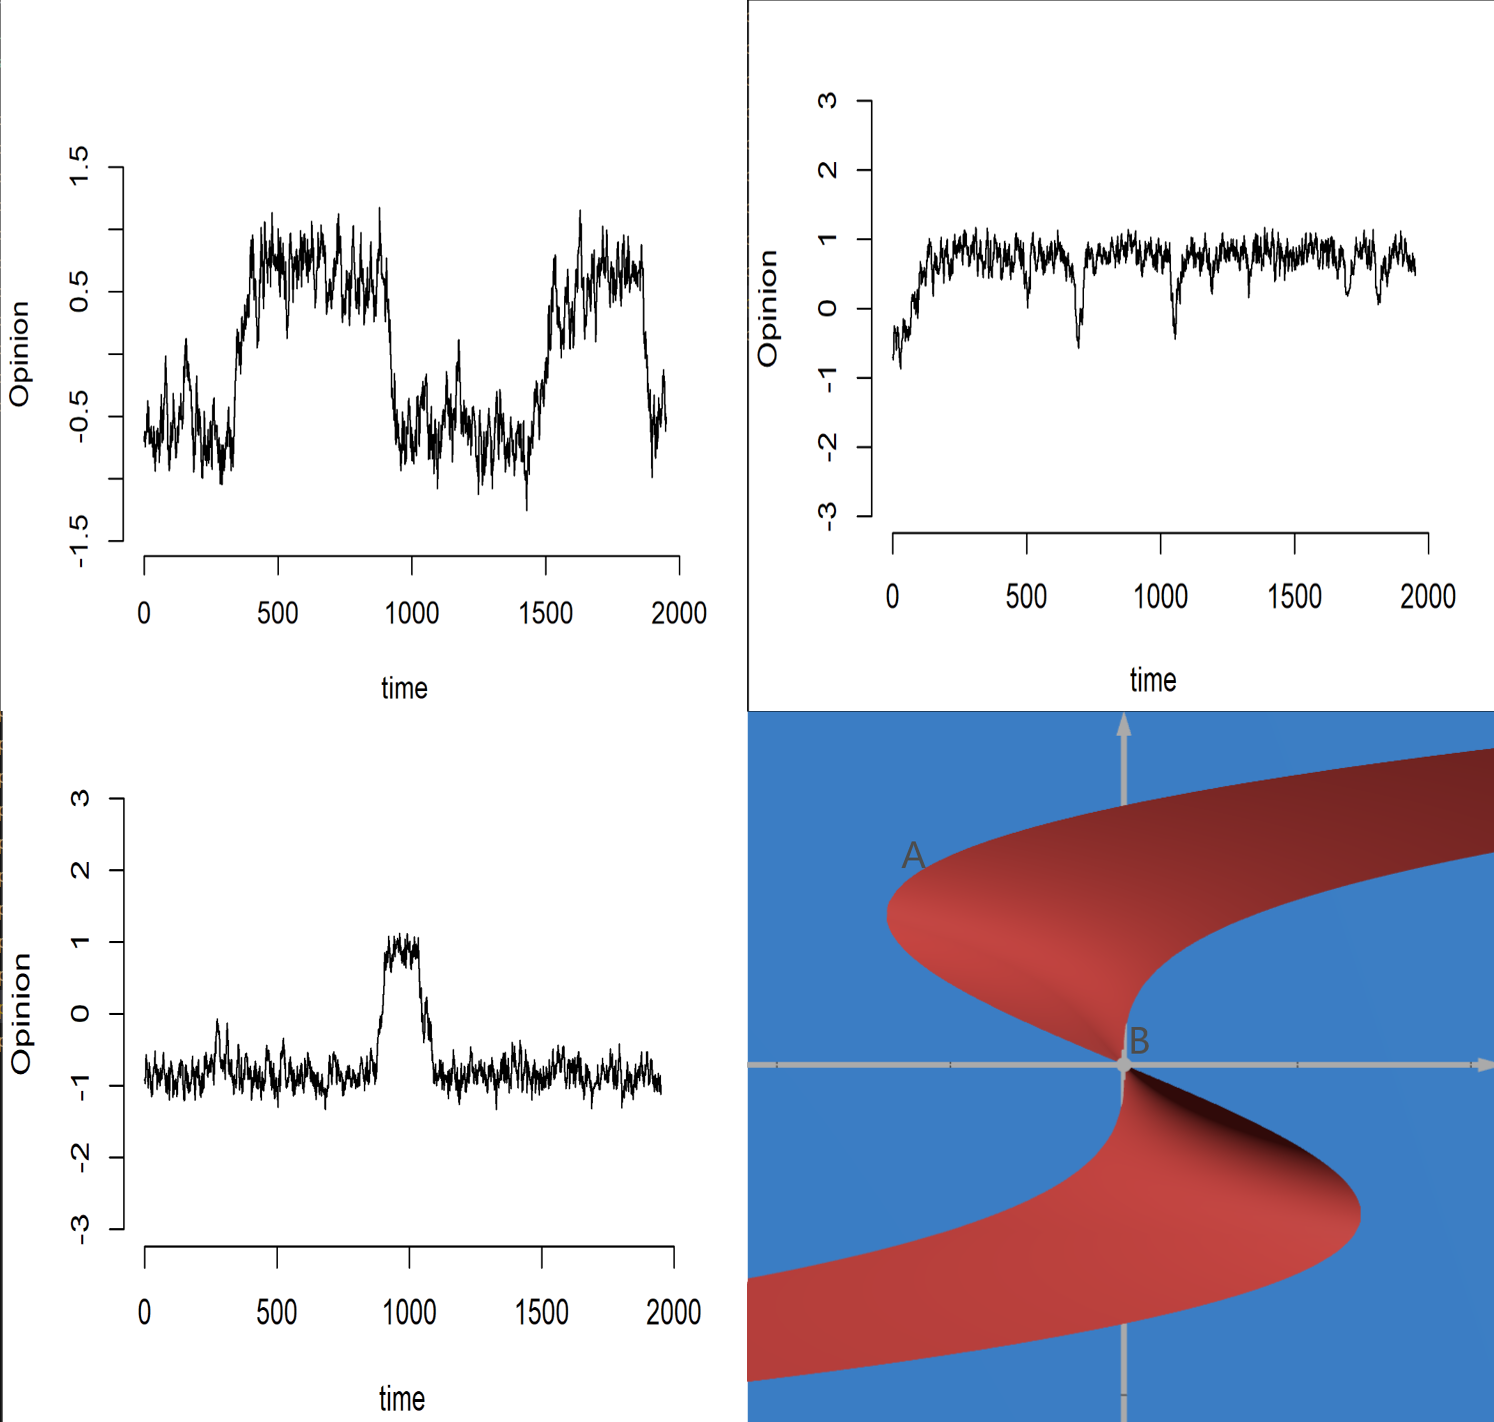
\includegraphics[width = 0.6\textwidth]{misc figure/combined_with_replacement.png}
    \caption{Sudden jump between bistable state due to noise. The top left figure shows sudden jumps of $O$ at $A=1,I=0$. The top right figure is $A=1,I=0.1$, opinion is much harder to stay in negative $O$ than the positive. The bottom left is $A=1.3,I=0$, sudden jumps occur rarer. The bottom right figure illustrate that at position A, which is negative $I$, the opinion is more likely to get over the unstable equilibrium surface, meaning that it is less likely to stay at positive opinion at that position.}
    \label{fig4}
\end{figure}

Noise appear in both update of opinion and information. Although opinion usually stay at one of the equilibrium surface in bistable area, sudden jumps to another equilibrium surface is possible if the noise of opinion $n_o$ accumulate to certain extent.
Recalling the cusp catastrophe, the unstable equilibrium surface is tilted in the middle, so at fixed $A$, different $I$ cause the opinion jump differently, meaning that at positive $I$, opinion stay at positive equilibrium surface more easily.
And for fixed $I$, the jumps occur rarer as increasing $A$, as a larger accumulated noise of opinion is required to get over the unstable equilibrium surface (\autoref{fig4}).\\

\begin{figure}[H]
    \centering
    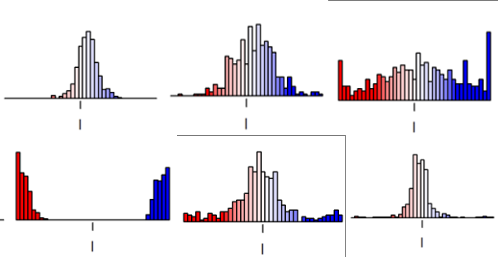
\includegraphics[width = 0.6\textwidth]{misc figure/spreadI.png}
    \caption{The upper part shows the spread of information distribution of agents solely due to noise (from left to right), no interaction is involved (the accumulation of information at $I=\pm1$ is because the plot include data points outside the $I$ axis and two ends, it is not polarization, information still spread evenly outside the $I$axis). The lower part shows the convergence of information when agents are initially having information of around $\pm 0.9$ evenly (from left to right), the information distribution converges at around 0 as iterations process. (stochastic block model is used)}
    \label{convergeofI}
\end{figure}

For the noise in information update, one interesting phenomenon is that the information of agents will diffuse  away along the information axis due to noise during iterations. The spread of information can cause change in stance after enough number of iterations even at $r_{min}=1$. In addition, we can derive from \autoref{eq5} that after enough iterations that agents keep interacting, the distribution of information
eventually converge together, implying an unimodal distribution of information, where the location of unimodal distribution depend on attention distribution. This means agents will have similar information in value, but polarization of opinion is still possible due to bistability (see \autoref{convergeofI}). A trouble of convergence of information is that it confines information distribution in a certain range, meaning that agents will always have
similar information when they are living together. However, this cannot explain the occurrence of activists with opposite information. In a society where information eventually converges, no new idea toward the attitude object can be generated. One method to solve the trouble is to introduce some 
potential activists with high noise in information, so that those potential activists still have chances to reach extreme information.\\


Attention also shows intriguing behaviors. During simulations, when $d_A$ is relatively small, the overall attention gathered at a value slightly lower than $A^*$, like there is a peak around $A^*$. Yet if $d_A$ is relatively large, the peak spread and shift towards 0, and a large fraction of agents having $A$ around 0 (see \autoref{attentionflow}).
This result can be explained in two aspects. First, larger $d_A$ leads to fast overall attention decay. Before an agent can interact again, large $d_A$ decrease attention rapidly thus further apart from $A^*$. Also, when $d_A$ is large, attention of agents can have better chance to go beyond the equilibrium, the larger the $d_A$, the further attention exceed $A^*$. This also implies that
attention of agents can move around the attention axis in a larger range with higher rate of change of $A$ if $d_A$ is high. Second, based on the selection rule in \autoref{eq3}, when $d_A$ is large,
after some iterations, a small group of agents will have attention much higher than the non-interacting agents, and the small group of agents will have much higher
possibility to be selected and boost their attention even more, resulting in even less chances for non-interacting agents to be selected, the gap in attention widened. This explains the residue at $A=0$.\\

\begin{figure}[H]
    \centering
    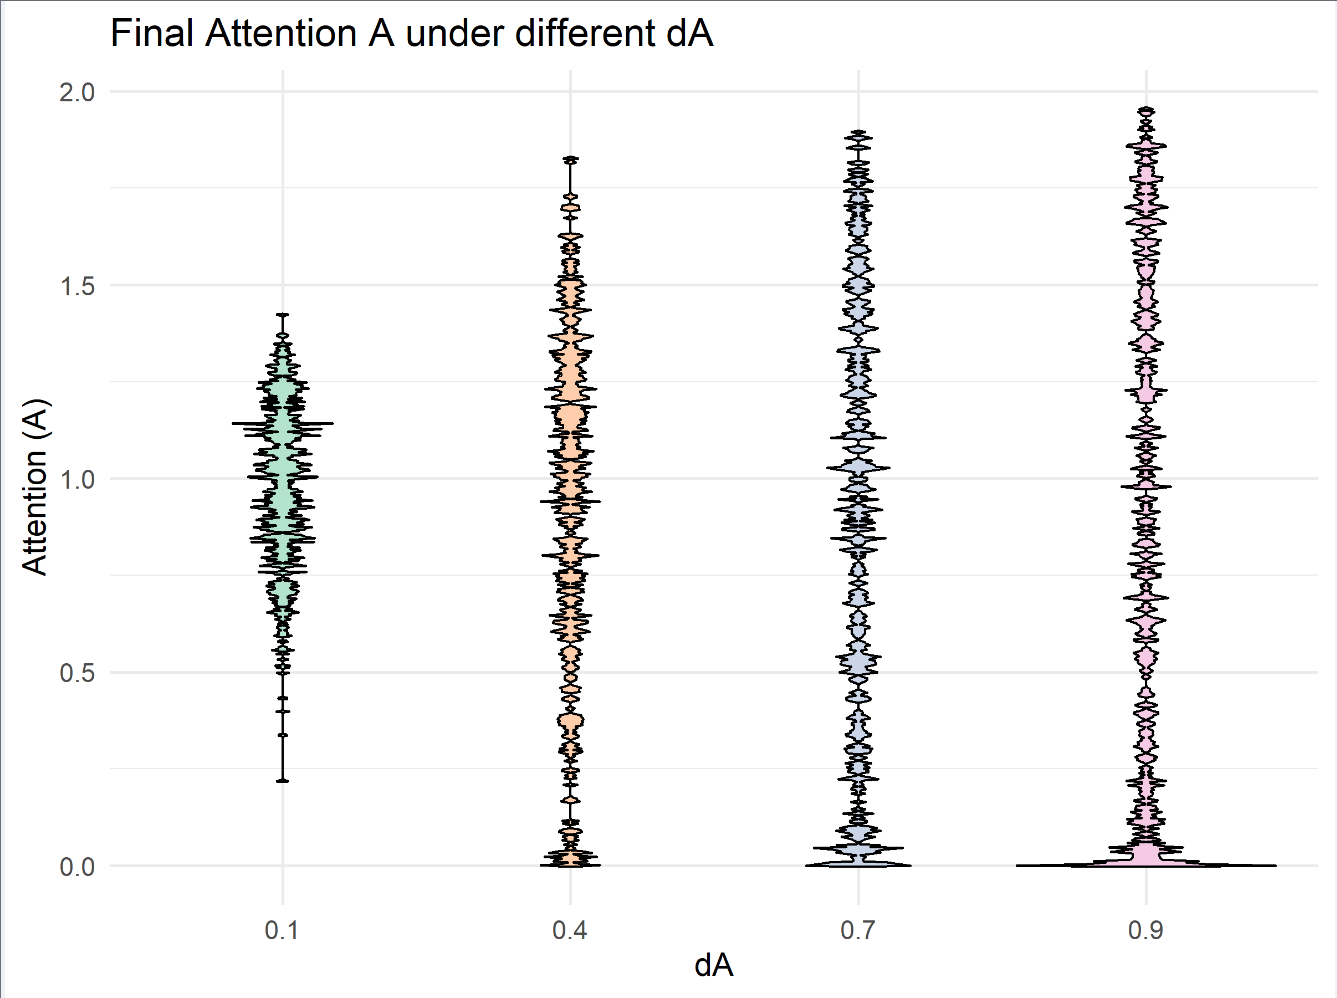
\includegraphics[width=0.6\textwidth]{misc figure/attentionflow.png}
    \caption{Distribution attention after 15000 iterations for different $d_A$. When $d_A$ is low, attention gathered around equilibrium. When $d_A$ is high, attention spread away and a fraction of agents having attention of 0.}
    \label{attentionflow}
\end{figure}

There are some hypotheses about $d_A$ here. $d_A$ represent the rate of change of attention. Based on \autoref{eq4}, it assumes that if one's attention is raised faster, his attention must decay at a higher rate when he is not think about the topic.
This resemble some real world situations. Recent studies point out that the attention span of the public toward an object in social media is shortening with steeper rate of change of attention through recent years\cite{lorenz2019accelerating}. As the accelerating information dissemination rate over past few years, we can know and receive information in a short time,
that helps us to raise our attention towards a topic more effectively. Hence we can interpret $d_A$ as something related to information dissemination rate in the society, not directly equal (information dissemination also affect $I$), but higher the information dissemination rate, higher the $d_A$ of the society. So the first hypothesis is a society with high information dissemination rate,
agents are more likely to have a shorter attention span on an attitude object, and for that attitude object, most agents eventually lost interest on it quickly and have weak stance on it due to low attention.\\

Another hypothesis is that when $d_A$ is too large, after some iteration, attention of an agent can become negative by using \autoref{eq4}. If $d_A$ is too large, attention can be boosted to a value much larger
than $A^*$ after an interaction, thus if $A>>A^*$ continued in second interaction, the term $d_A(2A^*-A)\delta$ become very negative, resulting a negative attention. The trouble is agent with negative attention can not be selected by \autoref{eq3}, it will be hard for the agent to escape negative attention unless his partner interact with him. Recall the Glauber dynamics, negative $A=\frac{1}{kT}$ indicates the system tends to increase its energy, leads to opposite spin with neighbour is preferred. 
In the Ising attitude model, negative $A$ means nodes are more likely to have opposite value with neighbours, resulting in $O\approx0$. This can be visualized in the cusp catastrophe also. The interpret of negative attention can be quite funny, 
it is like saying that if you force yourself to think about something too much in a short time, you will get negative attention and "overload", feeling so contradictory and giving up to have a stance. Similar phenomenon exists in real world. Exposure under massive information environment often cause cognitive overload and fatigue, leads to avoidance behavior that tends to delay or escape from making a decision or choosing a stance\cite{da2023cognitive,pilli2016information}. Although $\frac{1}{kT}$ is not likely to be negative,
but the mechanism of $A$ depends on \autoref{eq4}, so they are actually not identical, and the interesting one is that negative attention might could has meaning.
\section{Results}
In this section I will discuss some results produced in the article that are not explained in detail qualitatively.
\subsection{Black Pete}
According to the article, the Black Pete case show persuasive resistance be cause the uneven change in attention and information for each agent. Two activists with negative opinion, strong (negative) information and attention were intoduced to influence the majority, which is with low attention, positive information and opinion.. We can think of the position of an agent as a position vector $\vec{v}$, and the rate of change of the position vector
due to each interaction is $\vec{dv_i}=dI_i\hat{I} + dA_i\hat{A} + dO_i\hat{O}$ according to \autoref{eq5} ($dI_i$ here can mean change of information in one interaction, so it can be $dI_i = I_{i+1}-I_i$), \autoref{eq4} and \autoref{eq2}. In each interaction, $dA_i$ only depends on current attention but
$dI_i$ can depends on how far an agent at compare to activist. This is because $I_{i+1}$ is a weighted value between two agent's information, so agents near activists can have larger $dI_i$, while agents far away from activists receive information that is not so extreme, so $dI_i$ is smaller, this decay in $dI_i$ is due
to the weighted algorithm in change of information of agents. Recalling the cusp catastrophe in \autoref{fig1}, as an agent increasing his attention, the step size and the direction of $dI_i$ decide which equilibrium surface he will finally land.\\

\begin{figure}[H]
    \centering
    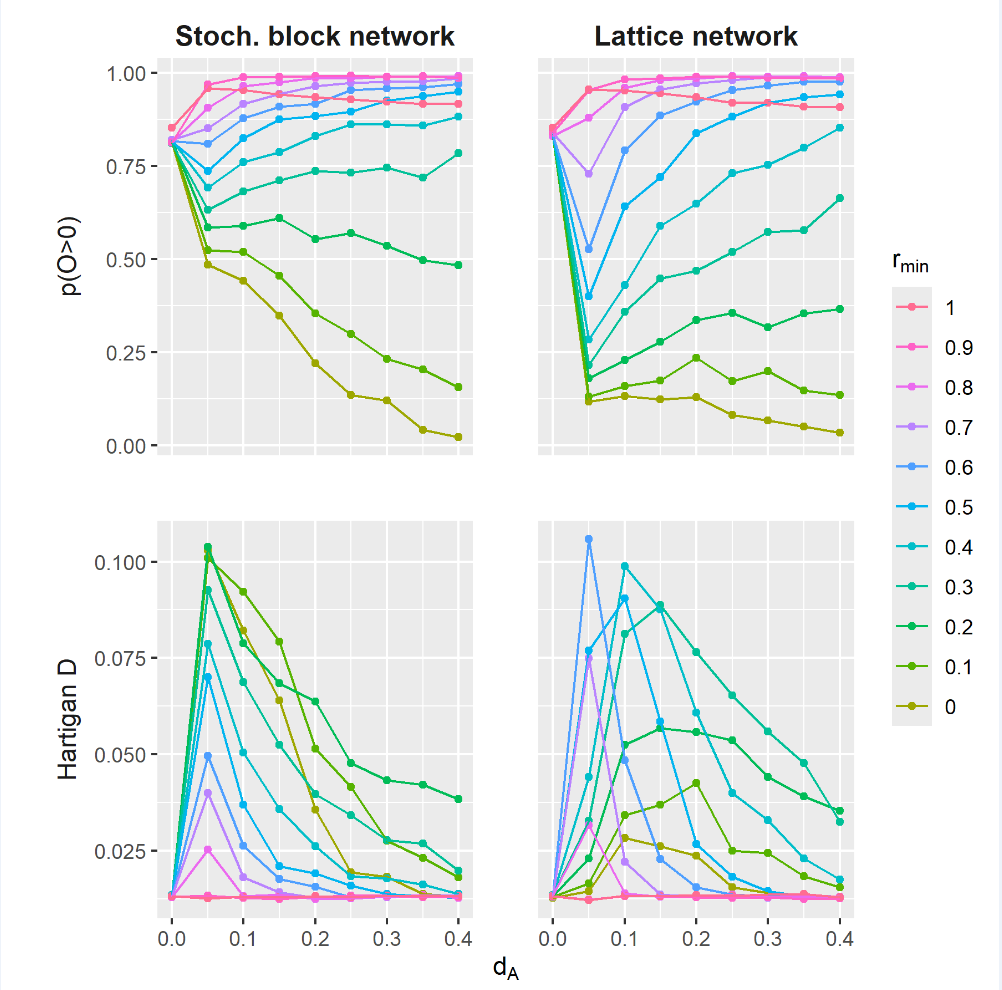
\includegraphics[width = 0.6\textwidth]{misc figure/fig6.png}
    \caption{Test of Black Pete case in different parameters. Results here is a bit different with the article one, which is because noise of information was adopted here, while not for the article.}
    \label{blackpete}
\end{figure}

The results of Black Pete under different parameters can be understand qualitatively by using some techniques mentioned in \autoref{Ext}. Different network models are used, but that does not affect the result too much. The network topology can affect the spreading speed of
information and attention, but not the fundamental mechanism. In actual quantification of the model, network topology might cause big differences in the work, but these are out of scope here.\\

In \autoref{blackpete}, we first look at the upper part. The behavior of $r_{min}=1$ curve was dominated by noise of information, and no information exchange also avoid converge of information. When $d_A=0$, there is no change for attention and information by interaction, but the information noise can spread away
and cause some position opinion of agents to switch their stance if they across the cusp line, this is more likely to happen for low attention agents (the majority), so $p(O>0)$ drops. When there is $d_A$ value, attention can increase so it will be more difficult
for agents to across the cusp line due to information noise (they have to move more distance to get across), we can obverse some lines, especially the $r_{min}=1$, increased suddenly at $d_A=0.05$. For such small value of $d_A$, a sharp peak was form at attention equilibrium, but as $d_A$ keep increasing,
attention of agents started to move around on the attention axis, and part of the agents having $A\approx0$. Higher $d_A$ leads to more fraction of agents having relatively low attention, the effect of information noise then affect the result again, causing drop in $r_{min}$ line in $p(O>0)$. For increasing trend of lines with high $r_{min}$ along $d_A$, at $d_A=0$,
since attention of the majority cannot be increased, activist drag the information of majority to their side very easily, so we see lower $p(O>0)$ than line $r_{min}=1$. As $d_A$ increase, attention of majority increase faster so that they can resist activists' persuasion better, that is the explanation for increasing $p(O>0)$. So, both $d_A$ and $r_{min}$ can affect
the persuasion efficiency by activists. This also explains higher $r_{min}$ can reach $p(O>0)\approx1$ faster at same $d_A$. For low $r_{min}$, agents can be persuaded by activist easily, this simply explain dropping $p(O>0)$ along $d_A$ and different $r_{min}$. For lower part, the Hartigan D is like reflecting $p(O>0)$ in an other way, the sudden increase at $d_A=0.05$ is just because activists drag agents to their side easily and low $d_A$
make attention of agents concentrated at $A^*$, which is overally high that opinion will be more extreme.

\subsection{Meat-eating vegetarian}
In the this case with bounded confidence $t_o$, $80\%$ of meat-eaters are low positive information and attention, and $20\%$ vegetarians are having high attention and strong negative information. With introduction of perturbation probability that can reverse the opinion of vegetarian, it is found that polarization can be reduced.

\begin{figure}[H]
    \centering
    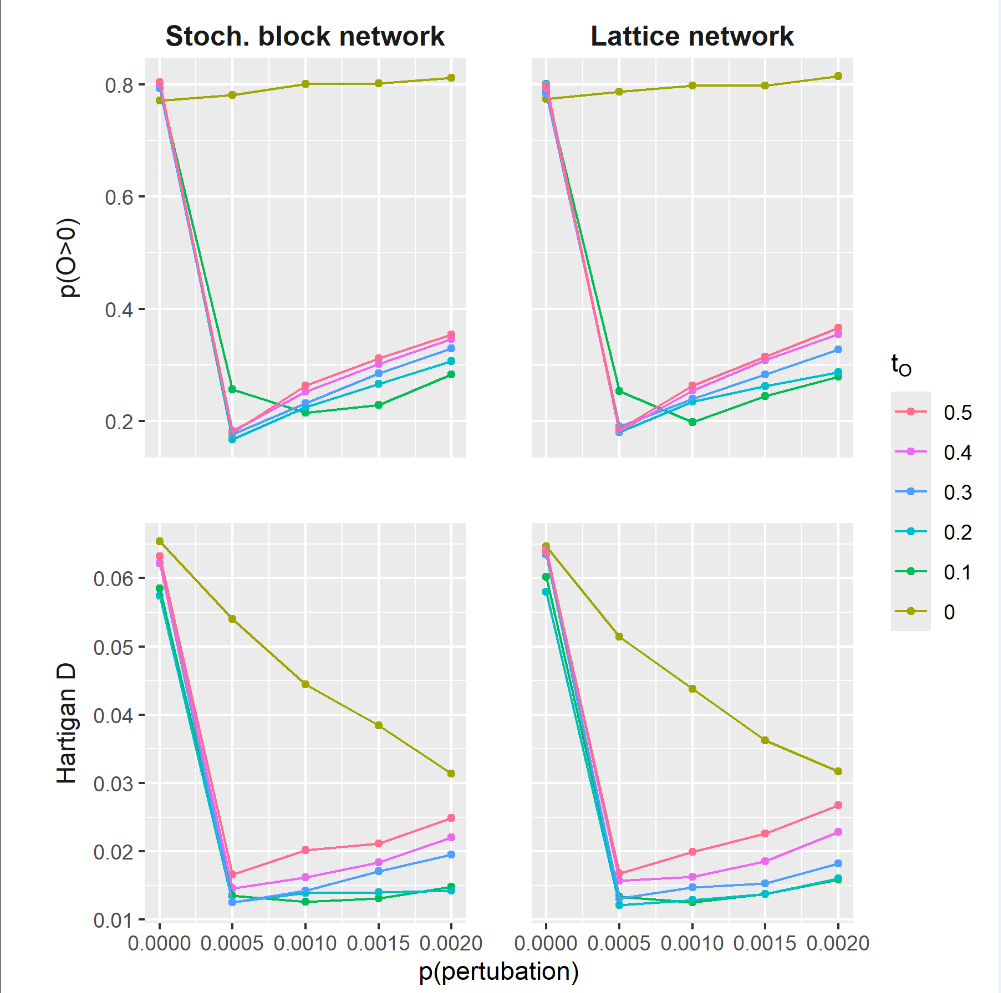
\includegraphics[width = 0.6\textwidth]{misc figure/fig8.png}
    \caption{Results of meat-eating vegetarian case under different parameters.}
    \label{meateat}
\end{figure}

Begin from upper part, when bounded confidence is 0, almost no interact can happen and contribute to change in information and attention. So the increasing trend in $t_o=0$ line along larger perturbation is just due to more vegetarian reversed their opinion to positive side, nothing more.
But we noticed at perturbation $=0$, $p(O>0)$ is slightly lower than 0.8, this is just because the noise of information and opinion. Meat-eaters with low attention and information get over the $O=0$ plane much more easier than vegetarians. For other $t_o$, agents of same opinions can interact, which avoid their
information to spread away due to noise, so at perturbation $=0$, they are closer to $p(O>0)=0.8$. When perturbation introduced, information exchange between opposite opinions is possible that information start to converge (thus depolarized). Since vegetarians have high attention and strong negative information, 
the converge point will be at area $I<0$, resulting to that more agents holds negative information and opinions. However, as perturbation probability increases, larger fraction of agents at negative opinion reverse their opinion to positive, leads to an increase in $p(O>0)$, this also explains the increasing Hartigan D.
For lower part, the Hartigan D just behave according to $p(O>0)$.\\

\subsection{Depolarization by $d_A$}
As discussed in \autoref{Ext}, larger $d_A$ allows agents move around in the attention axis faster and in larger range, and leaving part of agents having low attention. Depolarization is possible if we first converge information of all agents, then by making use of high $d_A$, let agents go to the low attention area and come back again, or just leave them at linear opinion area (which is at $A<0.5$ for $A_{min}=-0.5$), they will have opinions based to their information,
even in bistable area.

\begin{figure}[H]
    \centering
    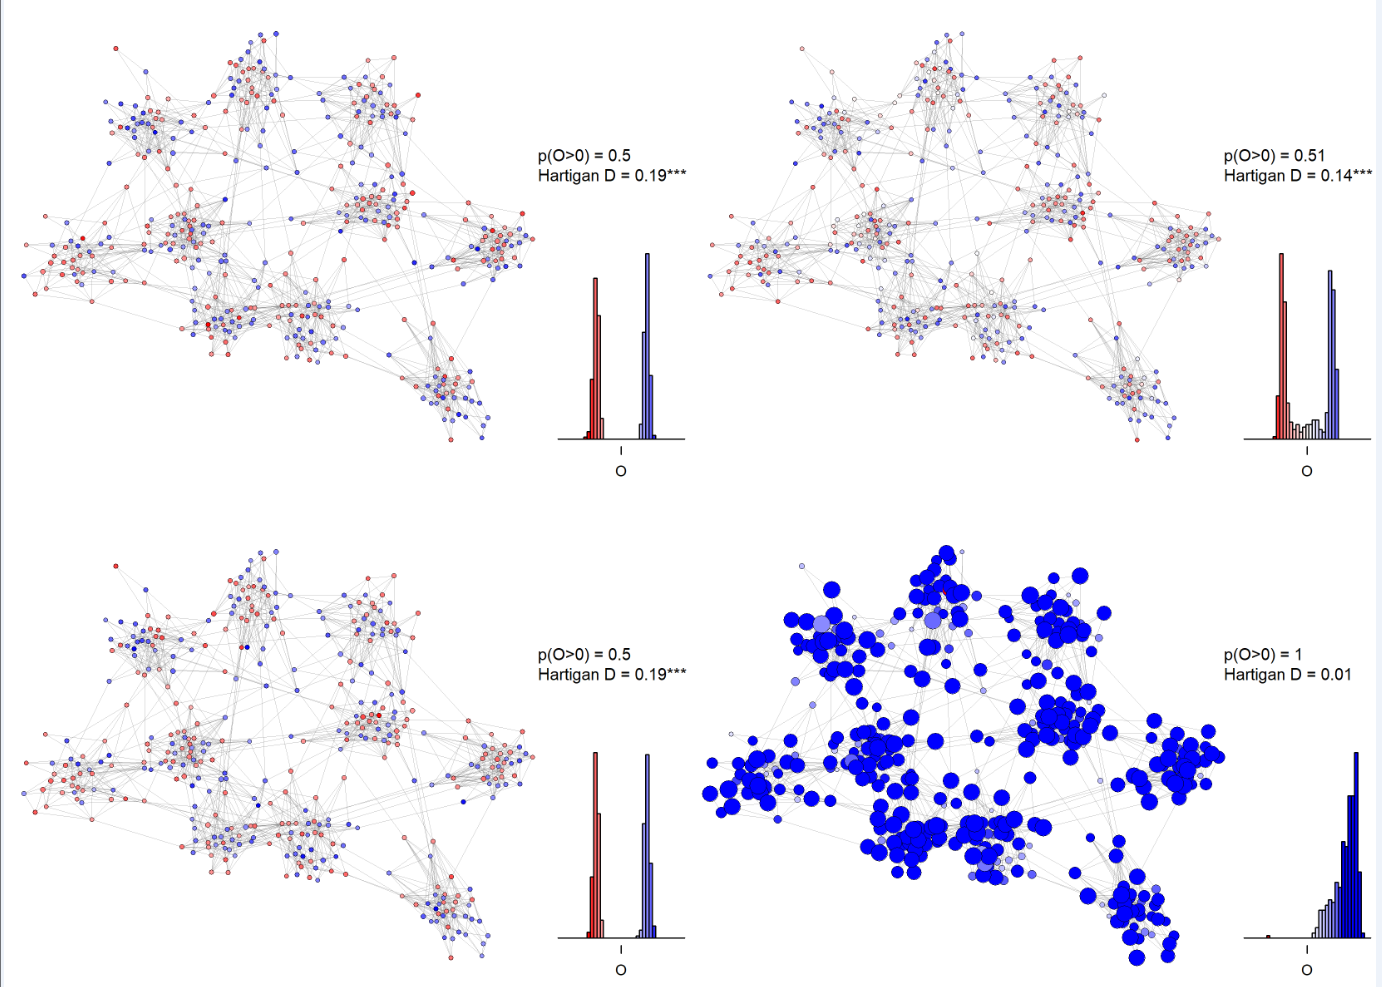
\includegraphics[width = 0.6\textwidth]{misc figure/depol.png}
    \caption{Depolarization by large $d_A$. Situation on the top has $d_A=0.1$, while the bottom one has $d_A=0.9$, other parameters are completely same. The size of nodes just represent the value of attention. }
    \label{depol}
\end{figure}

With parameter $n_s =0.0001,p=2,r_{min}=0.1,n_o=0.01,A^*=1,A_{min}=-0.5$, for top scenario, $d_A=0.1$, for bottom one, $d_A=0.9$, we can observe that polarization persist when $d_A$ is low, but if $d_A$ is high, polarization disappear and an unimodal distribution of opinions produced. This result shows that in a society with high $d_A$ (eg. fast information dissemination), people are more likely to have similar opinions with others, following what other says, and have relatively low attention to attitude objects (do not think much on a topic).
This might be a possible solution to reduce polarization in real world, not only because studies show that attention of people decrease if there is too much information\cite{pilli2016information}, but also we can interpret $d_A$ in real world as something related to information dissemination that we can manipulate.

\subsection{Diffusion pattern of activist}
In the Black Pete case, some parameters can affect the range that an activist can successfully persuade an agents. We can look more into it.

\begin{figure}[H]
    \centering
    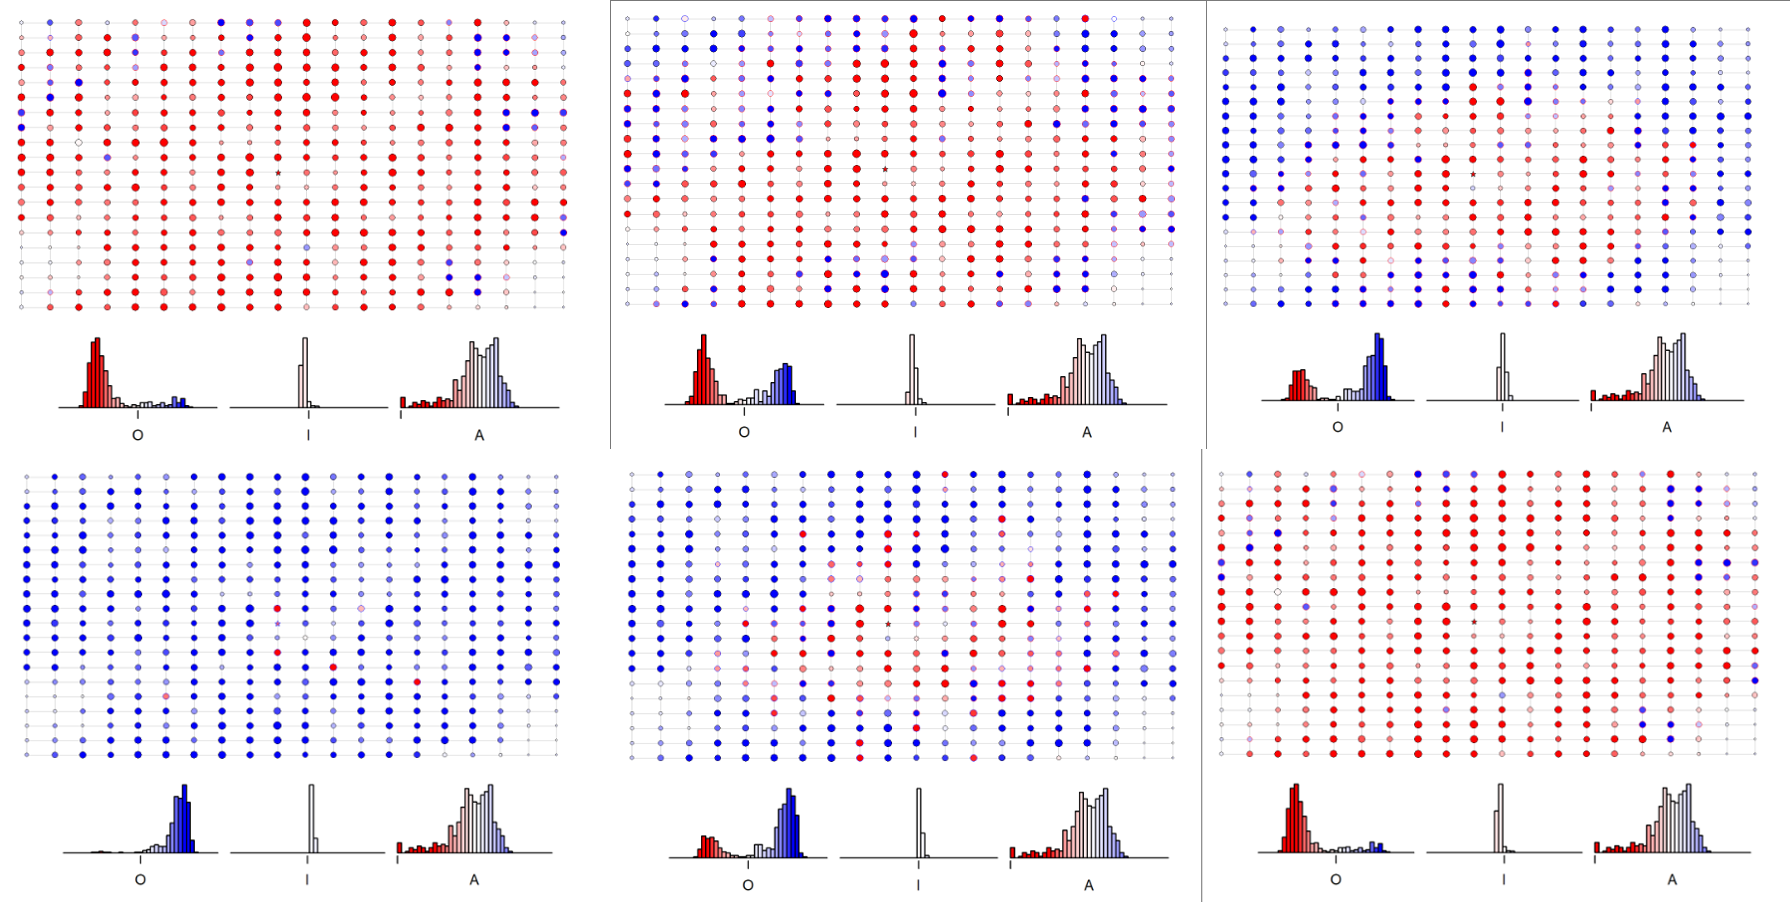
\includegraphics[width = 0.6\textwidth]{misc figure/combined_2x3.png}
    \caption{Parameters of $n_s =0,d_A=0.1,n_o=0.01,A^*=1,A_{min}=-0.5$ are used. The upper part shows when $p=2$, $r_{min}=0,0.2,0.4$ (left to right). The bottom shows at $r_{min}=0$, $p=1,1.5,2$ (left to right).}
    \label{diff}
\end{figure}

From the above results, we can see a qualitative trend as $p$ and $r_{min}$ increase, however, a quantitative method to indicate the result is not easy. We cannot just simply think about the distance
as not only the shape of diffusion is irregular, but also the emergence of agents with same stance with activist happen a bit randomly (red spot appear in somewhere surrounded by blue spot), making the diffusion is not so continuous.
But at least we are able to observe a trend and see parameters that affect the diffusion range visually. As $r_{min}$ and $p$ increase, activists are more difficult to affect other agents due to that they cannot influence their information effectively.

\section{Discussion}
As discussed in \autoref{Ext}, the inevitable convergence of information might be a problem. Other than having larger information noise, some modification on agents or interacting mechanisms can be further investigated. For exmaple, interaction between agents
with same stance can move their information to a more extreme stance. $d_A$ was discussed also, we mentioned that it is possible to have some relationship with information dissemination in real world. However, we still do not have a method to quantify a $d_A$ in real world (we do not know how fast information dissemination is in real world if $d_A=0.6$.), so empirical researches and quantification methods is needed
to make the HIOM more reliable, so that we know how a society is like specifically if $d_A=0.4$. Apart from $d_A$, we also need an explicit meaning in real world about other parameters, like $A^*$.\\

Although HIOM already show some interesting features like the cusp catastrophe, more modification can be made into the model based on emipical researches. Such as the network topology, connection between agents may change frequently, or agents can interact with each other simultaneously. The model restricted agents interact with each other one after another, interaction between multiple agents is impossible.
But in real situation, when a group of interact together, group polarization can occur that push their opinion into a more extreme degree\cite{moscovici1969group}. Another aspect is about individual agent. There is lack of evidence show that the process of forming an opinion equals solving for least energy as Ising model.
The thing is that we do not know how human mind works yet, and the proof is a really hard work, so we can now just pretend it as an assumption.

For the diffusion of activist, we can observe a range affected by activist visually, but quantifying it is need more research and methods, which we expect the work can be done in the future.

\section{Conclusion}
In this report, we try to understand the HIOM and analysis some parameters and mechanisms of it, including effect of noise, dynamics of $I$ and $A$. By looking further into these mechanisms, we raised a method to reduce polarization and tried to view the diffusion effect due to activists in Black Pete case. We also gave qualitative explanations to some results from the original article in order to have
deeper understanding in the HIOM.


















\bibliography{ref.bib}
\end{document}